\chapter{Matrice de vérification des performances}

La matrice de vérification des performances permet de visualiser les tests effectués sur le robot. Ces tests permettent de s'assurer que toutes les fonctionnalités cités par le DPF sont présentes dans le robot. Pour chaque sous-fonctionnalité, on y retrouve un ou plusieurs paramètres critiques associés ainsi que les tests effectués et les résultats obtenus.

\begin{figure}[h]
  \centering
  \caption{Matrice de vérification des performances}
  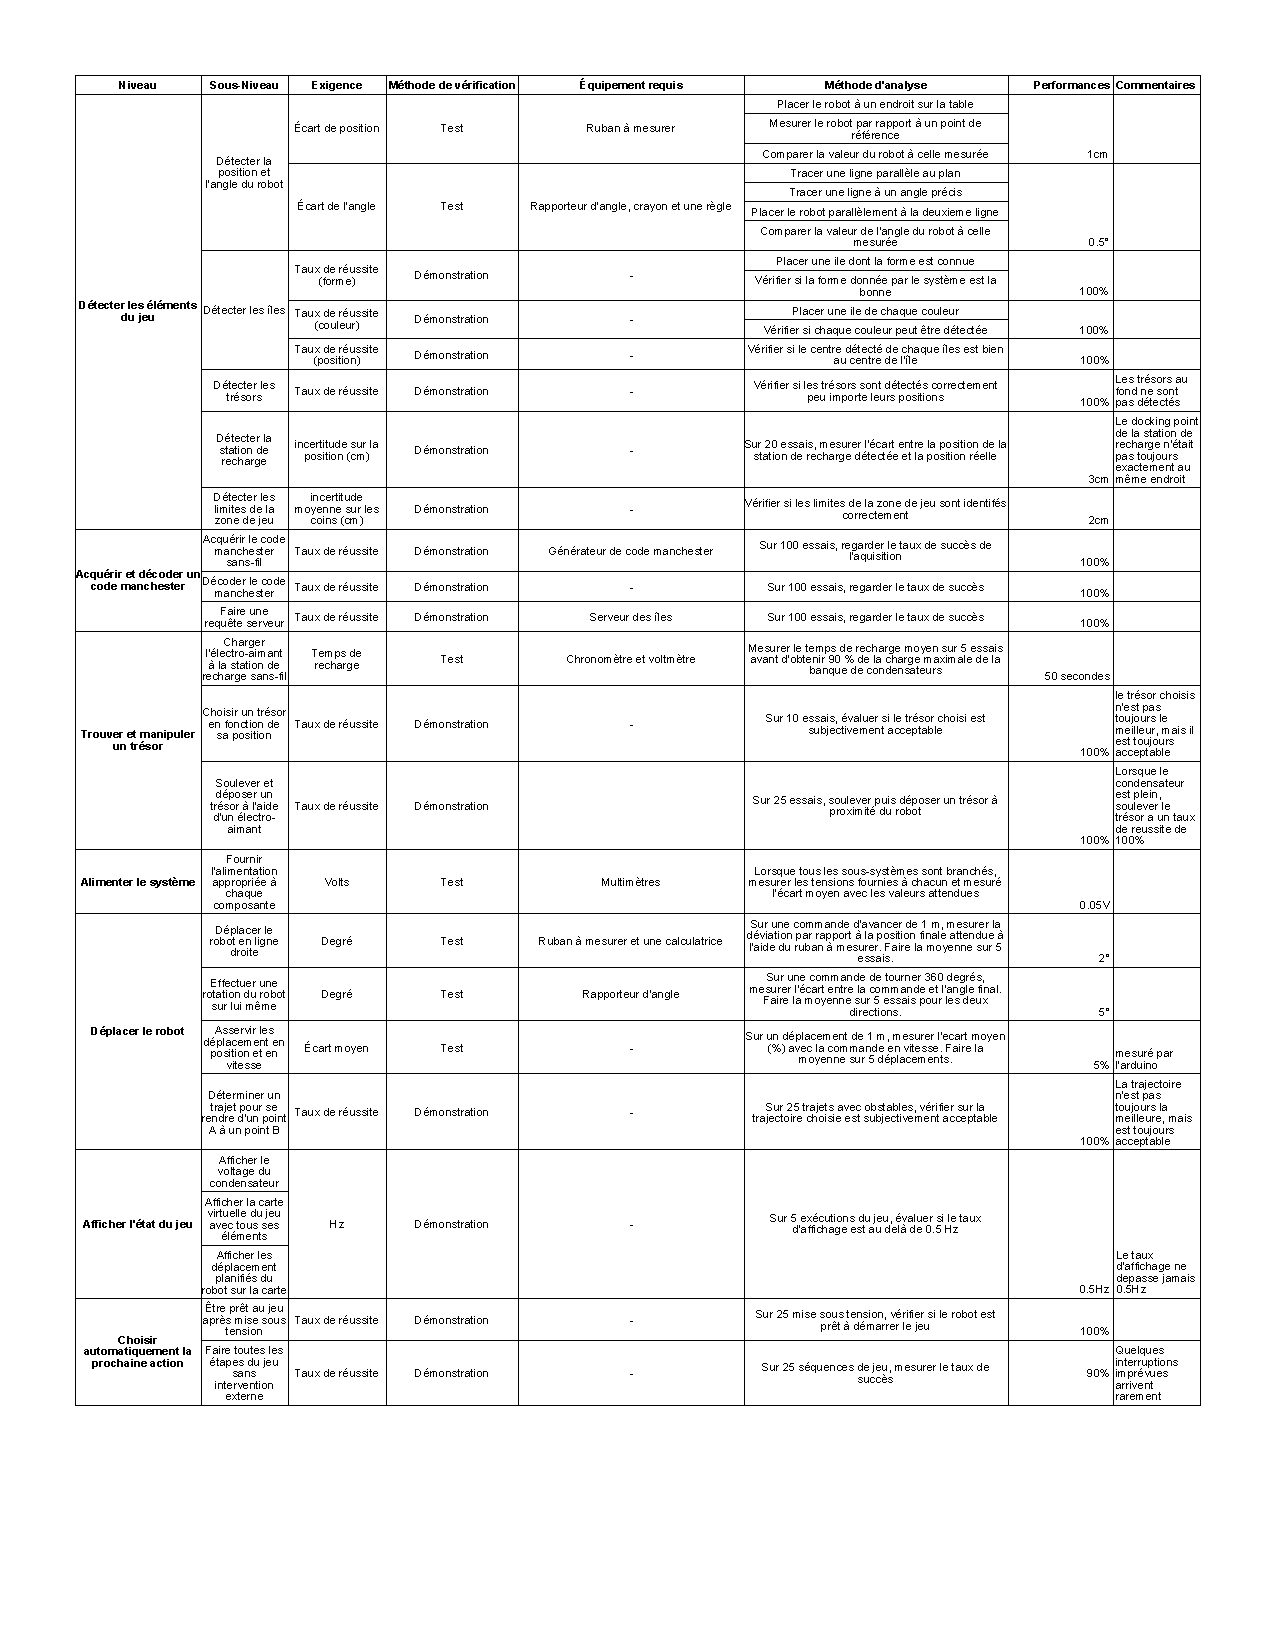
\includegraphics[scale=0.85]{resources/verification.pdf}
\end{figure}
